%template: https://www.sharelatex.com/templates/58d81eaaca5a6fd13992f8a4
\documentclass[12pt,letterpaper]{article}

\usepackage{cvpr}
\usepackage{times}
\usepackage{epsfig}
\usepackage{graphicx}
\usepackage{amsmath}
\usepackage{amssymb}
\usepackage[style=numeric]{biblatex}
\addbibresource{references.bib}
\usepackage{csquotes}
\usepackage{caption}

% Include other packages here, before hyperref.

% If you comment hyperref and then uncomment it, you should delete
% egpaper.aux before re-running latex.  (Or just hit 'q' on the first latex
% run, let it finish, and you should be clear).
\usepackage[breaklinks=true,bookmarks=false]{hyperref}

\cvprfinalcopy % *** Uncomment this line for the final submission

\def\cvprPaperID{****} % *** Enter the CVPR Paper ID here
\def\httilde{\mbox{\tt\raisebox{-.5ex}{\symbol{126}}}}

\linespread{1.5}
\setlength{\parindent}{2.5em}


% Pages are numbered in submission mode, and unnumbered in camera-ready
%\ifcvprfinal\pagestyle{empty}\fi
\setcounter{page}{1}
\begin{document}

%%%%%%%%% TITLE
\title{\textbf{ESC499 Interim Report:\\ \textit{Profiling GPU Memory with PyTorch}}}

\author{Author: Izaak Niksan\\
%Department of Computer Science, University of Toronto\\
%{\tt\small izaak.niksan@mail.utoronto.ca}\\
Supervisor: Prof. Gennady Pekhimenko\\
Advisor: Hongyu Zhu
}

\maketitle
%\thispagestyle{empty}

%%%%%%%%% INTRODUCTION
\section{Introduction}
Deep neural networks (DNNs) have a history dating back over half a century, with Donald Hebb's \enquote*{Hebbian Learning Rule} laying the foundations for modern techniques \cite{dnn_history}. In the proceeding years this approach was developed and improved, with notable developments by Rosenblatt (the first perceptron), Werbos (backpropagation), Jordan (Recurrent Neural Network), Hochreiter \& Schmidhuber (LSTM), and Hinton (Deep Belief Networks) \cite{dnn_history}. While this theoretical progression was occurring, the computational machinery required to actually implement these models was non-existent. In the last decade, the development of high-performance computing hardware - especially GPUs - has enabled many of these once-theoretical DNNs to be implemented in practice. Still, however, there remain bottlenecks which constrain implementations and therefore deeper insight into underlying resource usage is vital for further advancements in the field. \par 

%%%%%%%%% INTRODUCTION::Neural Networks
\cvprsubsection{Neural Networks}
While there are many types of neural networks, they all involve the transformation of some input data (for example the pixels of an image) into meaningful output - in fact, a neural network is nothing more than a composition of mathematical functions. The function modeled by a neural network is special, however, because it can model \textit{any} mathematical function with arbitrary accuracy (provided that the network has at least two layers) \cite{dnn_history}. It is because of this property that neural networks have been labeled \enquote*{universal approximators}. Loosely, this means that if there are useful patterns in the world - whether they correspond to user preferences in movies based on past movies they have watched, or classification of images based on their pixel composition, or even cardiac arrest likelihood based on heart rate - a sufficiently-trained neural network can identify it. The effectiveness of a neural network in identifying these patterns depends primarily on two things: the amount of data it has been trained with, and its specific topology.
\par

The neural network in Figure \ref{fig:feedforwardNN} shows the basic building blocks from which modern neural networks emerge. The green nodes represent the input data to the network, which is what the network must use to make meaningful predictions. Perhaps, the input vector $[x_1,x_2,x_3,x_4]^T$ might represent a four-word sentence.\par

The gray lines in the diagram represent \textit{weights}, or the scaling coefficients from one node to the next. These weights together create linear combinations of the outputs of one layer into the nodes of the next layer. \par 

The purple nodes represent \textit{neurons}, which take a weighted sum of input nodes and produce a scalar-valued output. Each neuron is a nonlinear function; the nonlinearity is important here because without it the universal approximator guarantees no longer apply. For example, each neuron might be the ReLU function $f(x)=max(x,0)$ which clips all negative values. Notice how there are two layers of purple nodes here - this denotes that the model has two hidden layers. There can be an arbitrary number of hidden layers in a network. \par 

Finally, the red nodes are the \textit{outputs}, which are the network's predictions based on the provided input data. In this example, each output node might be the one-hot-encoded representation of who likely wrote this sentence. If $y_1$ is associated with Alice, $y_2$ with Bob, and $y_3$ with Charlie, then the output vector $[y_1,y_2,y_3]^T = [0.983,0.217,0.015]^T$ indicates that it was likely Alice's sentence.

\begin{figure}[ht]
\centering
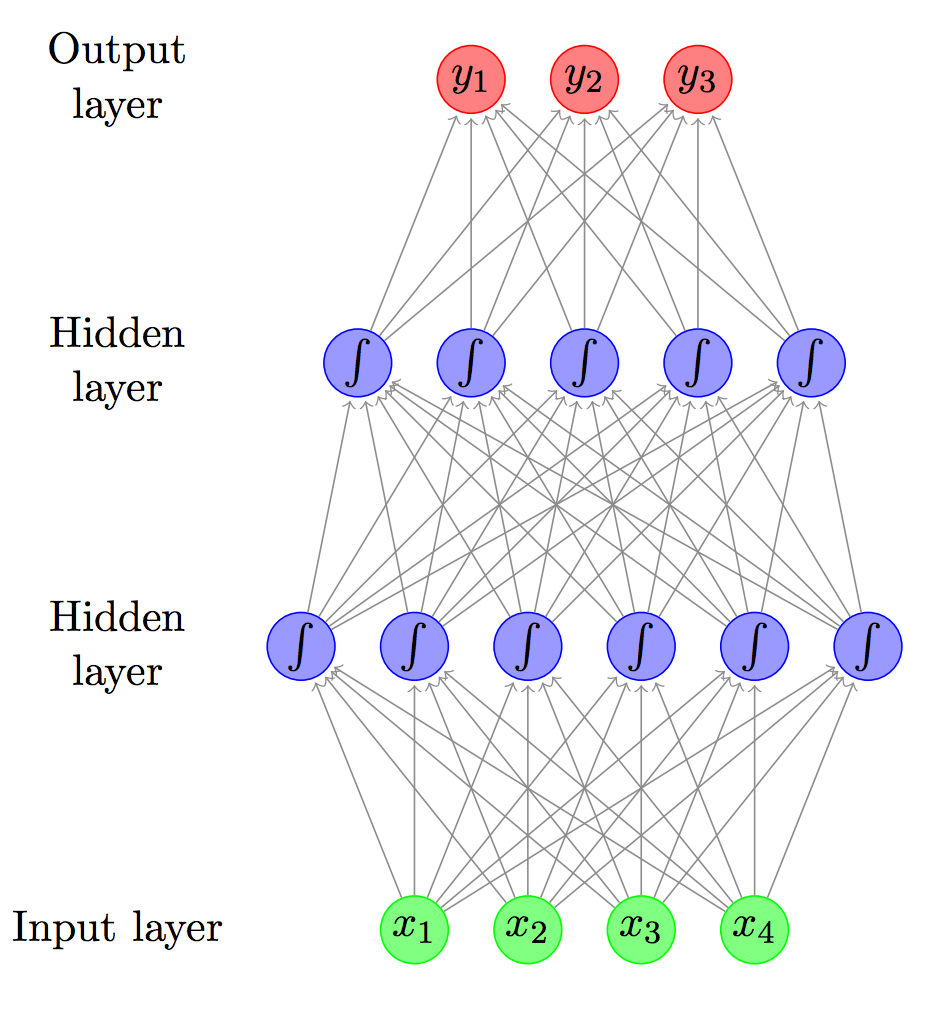
\includegraphics[width=0.4\textwidth,height=8cm]{neural_network_machinelearningmastery.png}
\captionsetup{width=0.7\linewidth}
\caption{ Topology of a fully-connected feedforward neural network \cite{feedforward_pic}}
\label{fig:feedforwardNN}
\end{figure}

%%%%%%%%% INTRODUCTION::GPUs and their application to DNNs
\cvprsubsection{GPUs and their application to DNNs}
Graphics Processing Units (GPUs) are at the center of recent machine learning breakthroughs. The computational workload for DNNs happens during \textit{training} (where DNNs are iteratively improved, e.g. to better-recognize faces or understand human speech) and \textit{inference}  (where already-trained DNNs are applied to the tasks they were trained for). Both training and inference are, in essence, complicated sequences of matrix operations; as it turns out, GPUs can perform these computations orders of magnitude faster than CPUs due to the parallelism inherent in their design. Figure \ref{fig:turing} shows the architecture of a modern GPU, which contains numerous computational cores (green).

\begin{figure}[ht]
\centering
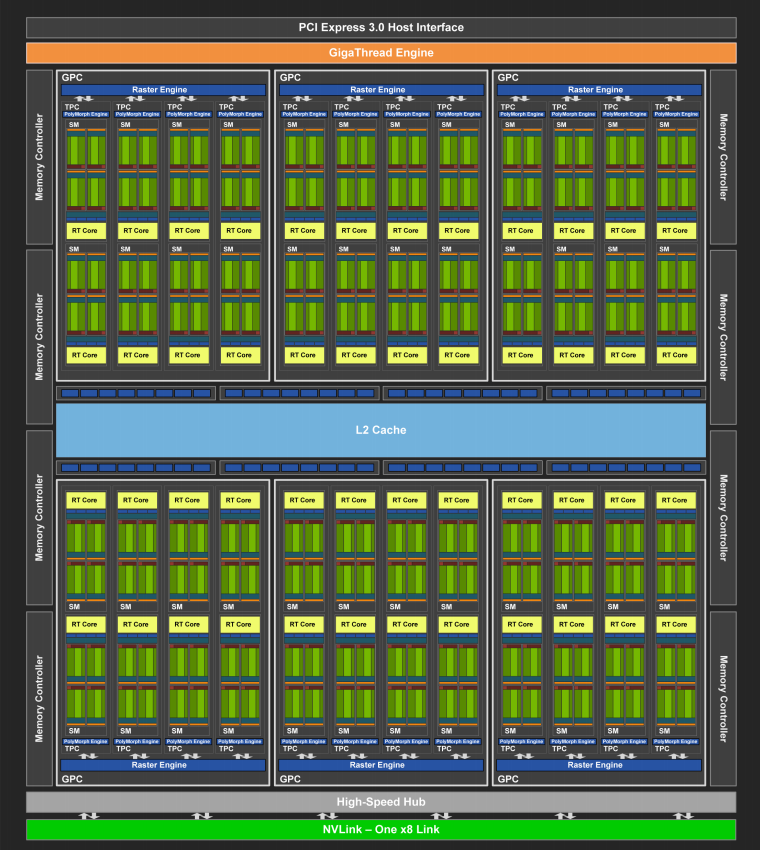
\includegraphics[width=0.7\textwidth]{Turing_TU104_chip_diagram.png}
\captionsetup{width=0.7\linewidth}
\caption{ Diagram of the NVIDIA Turing TU104 architecture. Green sections are CUDA cores, which together compose Streaming Multiprocessors (SMs) \cite{turing_architecture}}
\label{fig:turing}
\end{figure}

To understand the value that GPUs bring in terms of computational parallelism, suppose that a program is scaling a matrix as follows:
\[
3
\begin{bmatrix}
    a  &  b      \\
    c  &  d      
\end{bmatrix} 
=
\begin{bmatrix}
    3a  &  3b      \\
    3c  &  3d      
\end{bmatrix} 
\]
This computation can be distributed over 4 GPU cores, which would each scale one element of the matrix. The program can then accumulate the results of the four operations, and store the results either by overwriting the old matrix or by creating a new one in memory. While this is a small example, the same principles can be applied to matrices with thousands of elements - as the dimensions increase, so does the benefit of using GPUs. 
\par

NVIDIA conveniently provides the functionality to distribute a program's workload across GPU cores in the form of a rich C++ API \cite{cuda_guide}. This API can be integrated seamlessly into existing codebases in such a way that the programmer is abstracted away from the low-level architecture of the GPU they are using. In recent years, highly-tuned primitives for machine learning-specific applications (eg. convolution, softmax, batch normalization, neuron activations, etc.) have become publicly available \cite{cudnn}, which further allow programmers to use GPUs to their benefit.
\par 

%%%%%%%%% INTRODUCTION::Memory usage of DNNs
\cvprsubsection{Memory usage of DNNs}
One bottleneck which remains is the memory consumption of GPUs by DNNs. Inference requires an amount on the order of tens of MBs \cite{deep_compression}, while training might require tens of GBs \cite{vdnn}. NVIDIA’s RTX 2080 Ti comes with 11 GB of memory; even this modern, high-end device may face memory bottlenecks during training. \par 

In practice, DNNs are implemented via frameworks such as MXNet and PyTorch. These frameworks provide convenient interfaces which enable researchers to codify their DNN architecture in a language such as Python, abstracting away the low-level implementation details that would require GPU-specific programming experience. Despite the rise in popularity of these frameworks in recent years, comprehensive tools to understand their memory usage are not provided out of the box. The EcoSystem research team at UofT, led by Prof. Gennady Pekhimenko, has recently developed open-source memory profiling tools for MXNet, TensorFlow, and CNTK [4]; such a tool for PyTorch, however, remains to be created. PyTorch is increasingly becoming one of the most widely-used frameworks and thus a memory profiler would have a large impact to the community.
\par

Memory profilers provide otherwise-unavailable insight into how a framework handles the GPU’s memory and where it is being used (storing weights, gradients, feature maps, etc.). Understanding the memory breakdowns for various models drives the development of techniques that can optimize their footprints; some examples of existing techniques include Gist [5], vDNN [6], SCNN [7], and EIE [8]. Many of these developments were made possible in part due to detailed memory profiling functionality. 
\par

The first goal required for the development of a PyTorch memory profiler is to understand how PyTorch handles memory allocations at a low-level. The corresponding objectives will be to read the PyTorch codebase and get familiar with it, and then investigate how the framework allocates memory. The second goal is to create memory-profiling functionality for the framework. This is done by first modifying PyTorch to output logs during runtime about where and how memory is being used. It must be confirmed that all the expected memory is being accounted for, and that each allocation’s purpose is understood. Then, the memory allocations must be analyzed and visualized. The third goal is to use the PyTorch memory profiler in real-world use cases. This involves training cutting-edge models using the modified framework, reporting the results, and determining if improvements are possible.
\par

Changing the PyTorch framework involves altering the underlying C++ codebase. The source code is available publicly [9] and can be freely modified and rebuilt. A careful restructuring of this codebase will be required to ensure that every memory allocation is accounted for, and that it is known which data structures are requesting the memory. A parser program that will analyze the runtime outputs can be written in Python and, using libraries such as Matplotlib [10], a clear breakdown of the memory usage can be attained. Such a breakdown will include detailed information about how specific network layers and data structures consume memory.
\section{Literature Review}

\section{Progress to Date}


\section{Future Work}


\printbibliography
\end{document}